\documentclass[10pt]{beamer}
%\documentclass[handout,10pt]{beamer}
\usepackage{my_style}

%%%%%%%%%%%%%%%%%%%%%%%%%%%%%%%%%%%%%%%%%%%%%%%%%%%%%%%%%%%%%%%%%%%%%%%%
%%%%%%%%%%%%%%%%%%%%%%%%%%%%%%%%%%%%%%%%%%%%%%%%%%%%%%%%%%%%%%%%%%%%%%%%

\title[Math/CS 375]{Lecture 03 - B}
\subtitle{\S 4.3 Extrapolation}

\begin{document}
% -------------------------------------------------
\begin{frame}
  \titlepage
\end{frame}
% -------------------------------------------------

\begin{frame}{Goals}
We will answer these questions:\\[3mm]
\begin{itemize}
    \item What exactly is truncation error?
    \item What is Richardson extrapolation?
    \item What are the two sources of error when implementing a finite difference scheme on the computer?
    \item How do you approximate the 2nd derivative $f''(x)?$
\end{itemize}
\end{frame}

% ----------------
\sectionframe{Understanding Truncation Error}
% ----------------

\begin{frame}{Truncation Error}
    \begin{itemize}
        \item If we wrote the full Taylor series with no approximation
            \begin{equation*}
            f(x+h) = f(x) + h f'(x) + \frac{h^2}{2}f''(x) + \frac{h^3}{6}f'''(x)+\frac{h^4}{24}f''''(x)\cdots
            \end{equation*}
        \item Then rearranged to get forward difference 
            \begin{equation*}
            \frac{f(x+h) -f(x)}{h}=  f'(x) + \frac{h}{2}f''(x) + \frac{h^2}{6}f'''(x)+\frac{h^3}{24}f''''(x)\cdots
            \end{equation*}
        \item The error is $|$true$-$approx$|$
    \end{itemize}
    \begin{block}{Truncation Error}
    The truncation error is an \textit{infinite} series
        $$E=\frac{h}{2}f''(x) + \frac{h^2}{6}f'''(x)+\frac{h^3}{24}f''''(x)\cdots$$
    \end{block}
\end{frame}

%%%%%%%%%%%%%%%%%%%%%%%%%%%%%%%%%%%%%%%%%%%

\begin{frame}{Leading Order Term}

\begin{block}{Large $n$}
\begin{itemize}
    \item Recall that the worst-case 
    cost of bubble sort is 
    $$f(n) = \frac{n^2}{2}-\frac{n}{2}$$
    but we express this in Big-O notation as $\mO(n^2)$ as $n\rightarrow\infty$
    \vfill 
    \item When $n\gg0$, the $n^2/2$ term dominates the $n/2$ term
\end{itemize}
\end{block}

\onslide<2>{

\begin{block}{Small $h$}
\begin{itemize}
    \item  In the forward difference error        
    $$E=\frac{h}{2}f''(x) + \frac{h^2}{6}f'''(x)+\frac{h^3}{24}f''''(x)\cdots$$
    the term $h^2/2f''(x)$ dominates as $h\rightarrow0$ 
\end{itemize}
\end{block}
}
\end{frame}
% ----------------
\begin{frame}{Leading Order Term}

\begin{itemize}
    \item  If $h$ is small, then
    $$E=\underbrace{\frac{h}{2}f''(x)}_{\text{small}} + \underbrace{\frac{h^2}{6}f'''(x)}_{\text{tiny}}+\underbrace{\frac{h^3}{24}f''''(x)}_{very\; tiny}\cdots$$
    \vfill 
    \item In the limit $h\rightarrow0$ the term that dominates is 
    $$\frac{h}{2}f''(x)$$
    \vfill
    \item For \textbf{truncation error} we only care about the \textit{smallest} power of $h$ which in this case is
        $$E = \mO(h)$$
        \vfill
\end{itemize}
\end{frame}

\begin{frame}{Asymptotics}

\begin{itemize}
    \item Consider the function $f(x) = x + x^2 + x^3 $
    \vfill 
    \item In the limit as $x\rightarrow \infty$, 
    $$ f(x) = \mO(x^3)$$
    \vfill 
    \item In the limit as $x\rightarrow 0$, 
    $$f(x) = \mO(x)$$
    \vfill 
\end{itemize}

\keyidea{
When considering truncation error (small $h$) the term that vanishes the slowest is the leading order term.
}
    
\end{frame}

\begin{frame}{Main Idea}
\begin{itemize}
    \item We use Taylor expansions to derive equations such as
            \begin{equation*}
            \frac{f(x+h) -f(x)}{h}=  f'(x) + \frac{h}{2}f''(x) + \frac{h^2}{6}f'''(x)+\frac{h^3}{24}f''''(x)\cdots
            \end{equation*}
    \item<2-> Identify the true value, the approximation, and the error
    \begin{equation*}
            \underbrace{\frac{f(x+h) -f(x)}{h}}_{\text{approx}}=  \underbrace{f'(x)}_{\text{true}} + \underbrace{\frac{h}{2}f''(x) + \frac{h^2}{6}f'''(x)+\frac{h^3}{24}f''''(x)\cdots}_{\text{error}}
            \end{equation*}
    \item<3-> In the limit as $h\rightarrow 0$, the lowest power of $h$ dominates
        $$E=\underbrace{\frac{h}{2}f''(x)}_{\text{dominant}} + \underbrace{\frac{h^2}{6}f'''(x)+\frac{h^3}{24}f''''(x)\cdots}_{\text{asympototically insignificant}}=\mO(h)$$
    \vfill 
\end{itemize}
    
\end{frame}


% ----------------
\sectionframe{Extrapolation}
% ----------------

\begin{frame}{Improving the Method}

\begin{itemize}
    \item Suppose you want to approximate $f'(x)$
    \vfill 

    \item Suppose you already have one scheme $\phi(h)\approx f'(x)$ 
    \vfill

    \item For example $\phi(h)=\tfrac{f(x+h)-f(x)}{h}$
    \vfill
    \question{
  Can you develop an improvement $\psi(x)$ over the original $\phi$ using a linear combination, e.g. 
        $$\psi (h) = w_1 \phi(c_1 h) + w_2 \varphi(c_2 h)$$

    }
\end{itemize}
    
\end{frame}

\begin{frame}
\frametitle{Even Smarter?}
\begin{itemize}
    \item Let's try to improve centered difference
    \begin{equation*}
      \phi(h) = \frac{f(x+h) - f(x-h)}{2h} \approx f'(x)
    \end{equation*}
    \item<2-> We know that truncation error has \textit{even powers} of $h$
    \begin{align*}
      f'(x) & =  \frac{f(x+h) - f(x-h)}{2h} + c_2 h^2 + c_4 h^4 + c_6 h^6 + \dots\\
            & =  \phi(h) + c_2 h^2 + c_4 h^4 + c_6 h^6 + \dots\\
     \phi(h)& =  f'(x) - c_2 h^2 - c_4 h^4 - c_6 h^6 - \dots
    \end{align*}
    \item<3-> We expect the error to be reduced by 1/4 when $h$ is cut in half.
    \item<4-> Utilize this!
    \begin{align*}
     \phi(h)& =  f'(x) - c_2 h^2 - c_4 h^4 - c_6 h^6 - \dots\\
     \phi(h/2)& =  f'(x) - c_2 (h/2)^2 - c_4 (h/2)^4 - c_6 (h/2)^6 - \dots
    \end{align*}
\end{itemize} 
\end{frame}
%%%%%%%%%%%%%%%%%%%%%%%%%%%%%%%%%%%%%%%%%%%
\begin{frame}{Richardson Extrapolation}
\begin{itemize}
    \item Utilize this!
    \begin{align*}
     \phi(h)& =  f'(x) - c_2 h^2 - c_4 h^4 - c_6 h^6 - \dots\\
     \phi(h/2)& =  f'(x) - c_2 (h/2)^2 - c_4 (h/2)^4 - c_6 (h/2)^6 - \dots
    \end{align*}
    \item<2-> Combine these to eliminate the ``$c_2$'' term:
    \begin{equation*}
     \phi(h) - 4 \phi(h/2) =  -3 f'(x) - (3/4)c_4 h^4 - (15/16)c_6 h^6 - \dots
    \end{equation*}
    \item<3->Dividing by $-3$, and regrouping terms,
    \begin{equation*}
       \phi(h/2) + (1/3) \left( \phi(h/2) - \phi(h) \right) =  f'(x) + (1/4)c_4 h^4 + (5/16)c_6 h^6 - \dots
    \end{equation*}
    \item <4->Result: 
    \begin{equation*}
       \underbrace{\phi(h/2) + (1/3) \left( \phi(h/2) - \phi(h) \right)}_{\text{scheme}} =  \underbrace{f'(x)}_{\text{true}} + \underbrace{(1/4)c_4 h^4 + (5/16)c_6 h^6 - \dots}_{\text{error}}
    \end{equation*}
\end{itemize}
\end{frame}

%%%%%%%%%%%%%%%%%%%%%%%%%%%%%%%%%%%%%%%%%%%
\begin{frame}{Improvement in Accuracy}

    \begin{block}{Original Scheme}
    We started with $\phi(h)$ 2nd order accurate
        \begin{align*}
      f'(x) & =  \frac{f(x+h) - f(x-h)}{2h} + c_2 h^2 + c_4 h^4 + c_6 h^6 + \dots\\
            & =  \phi(h) + \mO(h^2)\\
    \end{align*}
    \end{block}

    \begin{block}{Fourth Order Richardson Extrapolation}
    We obtained $\psi(x)$ 4th order accurate
    \begin{align*}
     f'(x) &= \phi(h/2) + (1/3) (\phi(h/2) - \phi(h)) + (1/4)c_4 h^4 + (5/16)c_6 h^6 - \dots\\
    &= \psi(x) +\mO(h^4)
    \end{align*}
    \end{block}

    \keyidea{We eliminated the leading order error $c_2h^2$ to increase the accuracy.}
\end{frame}


%%%%%%%%%%%%%%%%%%%%%%%%%%%%%%%%%%%%%%%%%%%
\begin{frame}{And better?}

{
\question{What's stopping us from doing Richardson extrapolation again?}
}

\onslide<2->{
\begin{itemize}
    \item We can extend the Richardson extrapolation idea to any order.
    \item Idea: use $\psi(h) =  \phi(h/2) + (1/3) (\phi(h/2) - \phi(h))$ to
    annihilate the fourth order error term:
    \item<3-> Giving us 
    \begin{block}{Sixth Order Richardson Extrapolation}
    \begin{equation*}
      f'(x) = \psi(h/2) + (1/15)(\psi(h/2) - \psi(h)) + \mathcal{O}(h^6)
    \end{equation*}
    \end{block}
    where $\psi(h)$ is the fourth order Richardson extrapolation.
\end{itemize}
}
\end{frame}
%%%%%%%%%%%%%%%%%%%%%%%%%%%%%%%%%%%%%%%%%%%

\begin{frame}{Richardson Extrapolation}

    \begin{block}{Fourth Order Richardson Extrapolation}
    \begin{equation*}
     f'(x) = \phi(h/2) + (1/3) (\phi(h/2) - \phi(h)) + \mathcal{O}(h^4)
    \end{equation*}
    where $\phi(h)$ is the central difference approximation.
    \end{block}

        \begin{block}{Sixth Order Richardson Extrapolation}
    \begin{equation*}
      f'(x) = \psi(h/2) + (1/15)(\psi(h/2) - \psi(h)) + \mathcal{O}(h^6)
    \end{equation*}
    where $\psi(h)$ is the fourth order Richardson extrapolation.
    \end{block}
    
\method{Richardson Extrapolation}
{Derivative approximation $\phi(h) \approx f'(x)$}
{Improved approximation $\psi(h)$ }
{General technique to improve upon existing scheme.}
\end{frame}
%%%%%%%%%%%%%%%%%%%%%%%%%%%%%%%%%%%%%%%%%%%
\begin{frame}{Reduction of Error}
\begin{example}
    Suppose you use the 4th order Richardson to approximate $f'(x)$ with a small $h$ and you obtain the error $E$. How much smaller will the error be if $h$ is reduced by half?
\end{example}
\begin{itemize}
    \item We begin by finding a formula for $E$
    $$E = \mO(h^4) \approx Ch^4 $$

    \item If we halve $h$ then 
    $$E_{1/2} = O((h/2)^4) \approx C \frac{h^4}{2^4}=C\frac{h^4}{16}$$

    \item Since $E=Ch^4$ we have 
    $$E_{1/2} = \frac{Ch^4}{16} = \frac{E}{16}$$
    so $E_{1/2}$ is \textit{sixteen} times smaller than $E$
\end{itemize}
\end{frame}


%%%%%%%%%%%%%%%%%%%%%%%%%%%%%%%%%%%%%%%%%%%
\sectionframe{Rounding vs. Truncation Error}
%%%%%%%%%%%%%%%%%%%%%%%%%%%%%%%%%%%%%%%%%%%
\begin{frame}{Numerical Test, \texttt{diff\_richard.m}}
\begin{itemize}
    \item Consider
    \begin{equation*}
      f(x) = \sin(\pi x)\,\, \text{on}\,\, [-1,1]
    \end{equation*}
    \item Run code to approximate $f'(x) = \pi \cos(\pi x)$ using
    \begin{equation*}
      f'(x) = \phi(h/2) + (1/3) (\phi(h/2) - \phi(h)) + \mathcal{O}(h^4)
    \end{equation*}
    with
    $$h=0.01$$
    \bigskip
    
    \item<2-> We see that $p\approx 3.9999$, so its $O(h^4)$ accurate!
    
    \item<3-> Next lower stepsize to $h=0.001$ 
\end{itemize}
\onslide<4>{
\begin{alertblock}{!!!}
    Decreasing $h$ to $0.001$ made the error \emph{worse} instead of improving it!
\end{alertblock}
}
\end{frame}

\begin{frame}{Truncation Error}

\begin{block}{Truncation Error}
\begin{itemize}
    \item \textbf{Definition:} The error that arises when an infinite series is approximated by a finite sum.

\item \textbf{Example:} Using the forward difference formula:
\begin{equation*}
    f'(x) = \frac{f(x+h) - f(x)}{h} - \frac{h}{2} f''(\xi)
\end{equation*}
The term $- \frac{h}{2} f''(\xi)$ represents truncation error.

\item \textbf{How to Reduce:} Use higher-order methods such as the central difference or Richardson extrapolation.
\end{itemize}
\end{block}
\begin{center}
    Truncation error is a mathematical error introduced in the development of the scheme.
\end{center}

\end{frame}


\begin{frame}{Rounding Error}
    \begin{block}{Rounding Error}
    \begin{itemize}
        \item \textbf{Definition:} The error due to finite precision arithmetic in computers, which leads to small inaccuracies in calculations.

\item \textbf{Example:} If $h$ is too small, subtracting nearly equal numbers (e.g., $f(x+h) - f(x)$) can lead to significant loss of precision due to floating-point rounding errors.

\item \textbf{How to Reduce:} Choose an optimal step size $h$—not too large (to minimize truncation error) and not too small (to minimize rounding error).
    \end{itemize}
\end{block}
\begin{center}
    Rounding error is a numerical error introduced in the implementation of the scheme.
\end{center}
\end{frame}

\begin{frame}{Caution About Tuning $h$}

\begin{figure}
    \centering
    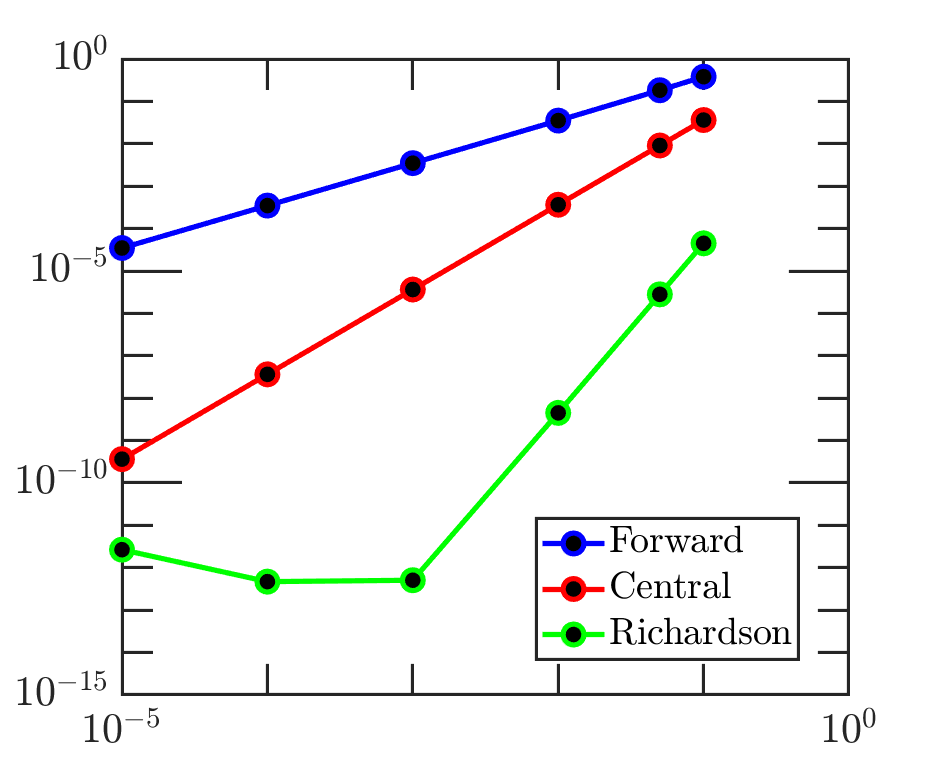
\includegraphics[width=0.5\linewidth]{figs/rich_comparison.png}
    % \caption{Caption}
    % \label{fig:enter-label}
\end{figure}
\begin{itemize}
    \item Richardson error converges to zero the \underline{most rapidly} 
    \item Richardson error starts to \underline{rise} after going lower than critical value of $h$
    \item The error computed in Matlab contains a mix of truncation error \underline{AND} rounding error
\end{itemize}
\end{frame}
%-------------------
\begin{frame}{Total Error}

\begin{itemize}
    \item \textbf{Truncation Error} is theoretical 
    $$ E_{\text{trunc}} = \left|f'(x) - \frac{f(x+h)-f(x)}{h}\right|$$
    \item \textbf{Round-off Error} happens when you use floating-point numbers
    $$ E_{\text{round}} = \left|\frac{f(x+h)-f(x)}{h} - \textrm{fl}\left(\frac{f(x+h)-f(x)}{h}\right)\right|$$
    \item The total error is the sum of both errors 
    $$ E_{\text{total}} = E_{\text{trunc}} + E_{\text{round}}$$
\end{itemize}

    
\end{frame}


%-------------------




\begin{frame}{Total Error}
\begin{block}{Total Error}
Approximating $f'(a)$ on the computer will contain a mixture of truncation error \textit{and} rounding error.
\end{block}

\vspace{3mm}

\keyidea{
The truncation error decreases as we make the parameter $h$ smaller. However, when $h$ is too small rounding error will take over and cause the error to rise.
}

\onslide<2->{
\textit{How do you know how small to make $h$?}
}
\onslide<3>{
\textbf{Homework!}
}
\end{frame}

%%%%%%%%%%%%%%%%%%%%%%%%%%%%%%%%%%%%%%%%%%
\sectionframe{Second Order Derivative}
%%%%%%%%%%%%%%%%%%%%%%%%%%%%%%%%%%%%%%%%%

\begin{frame}{Derivative Approximations}

\begin{block}{Forward Difference}
    $$f'(x) \approx \frac{f(x+h)-f(x)}{h}$$
\end{block}

\begin{block}{Backward Difference}
    $$f'(x) \approx \frac{f(x)-f(x-h)}{h}$$
\end{block}

\begin{block}{Central Difference}

    $$f'(x) \approx \frac{f(x+h)-f(x-h)}{2h}$$
\end{block}


\question{
\begin{center}
How do we approximate $f''(x)?$
\end{center}
}

\end{frame}

\begin{frame}{Derivation}
\begin{itemize}
    \item Look at the Forward AND Backward Taylor series together
    \begin{align*}
      f(x+h) & = f(x) + h f'(x) + \frac{h^2}{2}f''(x) + \frac{h^3}{6}f'''(x) + \frac{h^4}{24}f''''(\xi_{+})\\
      f(x-h) & = f(x) - h f'(x) + \frac{h^2}{2}f''(x) - \frac{h^3}{6}f'''(x) + \frac{h^4}{24}f''''(\xi_{-})\\
    \end{align*}

    \item<2-> Add them:
    \begin{equation*}
      f(x+h) + f(x-h) = 2 f(x) + h^2f''(x) + \frac{h^4}{12}f''''(\xi)
    \end{equation*}
    \item<3-> Subtract
    \begin{equation*}
      f(x+h) + f(x-h) -2f(x)= h^2f''(x) + \frac{h^4}{12}f''''(\xi)
    \end{equation*}
    \item<4-> Divide
    \begin{equation*}
      \frac{f(x+h) + f(x-h) -2f(x)}{h^2}= f''(x) + \frac{h^2}{12}f''''(\xi)
    \end{equation*}
\end{itemize}
\end{frame}
%%%%%%%%%%%%%%%%%%%%%%%%%%
\begin{frame}{2nd Order Central Difference}

\begin{block}{Scheme}
    $$f''(x) = \underbrace{\frac{f(x+h)-2f(x)+f(x-h)}{h^2}}_{\text{scheme}} + \underbrace{\frac{h^2}{12}f''''(\xi)}_{\text{error}}$$
\end{block}

\method{2nd Order Central Difference}
{function $f(x)$, step parameter $h$}
{approximation to $f''(x)$}
{This scheme approximates $f''(x)$ knowing nothing about $f'(x)$}

\vfill
\textbf{Note:}
Since the error term contains $f''''(\xi)$ this formula has \textit{zero error} if $f(x)$ is a 3rd order polynomial.
\end{frame}


%%%%%%%%%%%%%%%%%%%%%%%%%%%%%%%%%%%
\sectionframe{Hand Calculations}
%%%%%%%%%%%%%%%%%%%%%%%%%%%%%%%%%%%

\begin{frame}{Forward Difference}
\begin{example}
Approximate $f'(1)$ for $f(x)=x^3$ using the forward difference with $h=\tfrac12$.
\end{example}

\begin{itemize}
    \item True derivative:
    \[
    f'(x) = 3x^2 \quad \Rightarrow \quad f'(1)=3
    \]

    \item Forward difference:
    \[
    f'(1) \approx \frac{f(1+h)-f(1)}{h}
    \]

    \item Compute:
    \[
    \frac{(3/2)^3 - 1^3}{1/2}
    = \frac{\frac{27}{8}-1}{1/2}
    = \frac{\frac{19}{8}}{1/2}
    = \frac{19}{4}
    = 4.75
    \]

    \item Error:
    \[
    |4.75 - 3| = 1.75
    \]
\end{itemize}

\keyidea{Forward difference can be very inaccurate for moderate $h$.}
\end{frame}


\begin{frame}{1st Order Central Difference}
\begin{example}
Approximate $f'(1)$ for $f(x)=x^3$ using the central difference with $h=\tfrac12$.
\end{example}

\begin{itemize}
    \item Central difference:
    \[
    f'(1) \approx \frac{f(1+h)-f(1-h)}{2h}
    \]

    \item Compute:
    \[
    \frac{(3/2)^3 - (1/2)^3}{1}
    = \frac{\frac{27}{8}-\frac{1}{8}}{1}
    = \frac{26}{8}
    = \frac{13}{4}
    = 3.25
    \]

    \item Error:
    \[
    |3.25 - 3| = 0.25
    \]
\end{itemize}


\end{frame}


\begin{frame}{Comparison}
\begin{block}{Problem}
    Approximate $f'(1)$ for $f(x)$ using $h=1/2$.
\end{block}
\begin{center}
\begin{tabular}{c|c|c}
Method & Approximation & Error \\
\hline
Forward Difference & $\frac{19}{4}$ & $1.75$ \\
Central Difference & $\frac{13}{4}$ & $0.25$
\end{tabular}
\end{center}

\vspace{4mm}

\keyidea{Central difference is much more accurate at the same $h$.}
\end{frame}


\begin{frame}{2nd Order Central Difference}
\begin{example}
Approximate $f''(1)$ for $f(x)=x^3$ using the second-order central difference with $h=\tfrac12$.
\end{example}

\begin{itemize}
    \item True second derivative:
    \[
    f''(x) = 6x \quad \Rightarrow \quad f''(1)=6
    \]

    \item Approximation:
    \[
    f''(1) \approx \frac{f(1+h)-2f(1)+f(1-h)}{h^2}
    \]

    \item Compute:
    \[
    \frac{\frac{27}{8}-2(1)+\frac{1}{8}}{(1/2)^2}
    = \frac{\frac{28}{8}-2}{1/4}
    = \frac{3.5 - 2}{1/4}
    = \frac{1.5}{1/4}
    = 6
    \]
\end{itemize}
\onslide<2>{
\begin{center}
    There is NO error for approximating the derivative!
\end{center}
}
\end{frame}

\begin{frame}{Why is there no error?}

\begin{block}{Scheme}
    $$f''(x) = \underbrace{\frac{f(x+h)-2f(x)+f(x-h)}{h^2}}_{\text{scheme}} + \underbrace{\frac{h^2}{12}f''''(\xi)}_{\text{error}}$$
\end{block}
\begin{itemize}
    \item The leading order term contains $f''''(\xi)$

    \item The function we approximated was $f(x)=x^3$

    \item The derivatives are:
    \begin{align*}
        f'(x) &= 3x^2\\
        f''(x) &= 6x\\
        f'''(x) &= 6\\
        f''''(x) &= 0
    \end{align*}
\end{itemize}
\onslide<2>{
\keyidea{
The central difference will never have any truncation error if the function is a polynomial of degree 3 or less.
}
}
\end{frame}
\end{document}
